\chapter{Conjuntos Numéricos}
\section{Introdução}

A criação dos números, como conhecemos hoje, é produto da evolução de ideias sobre como representar determinadas grandezas, resolver problemas geométricos, problemas aplicados às ciências e resolução de equações. 

A noção de número inteiro foi criada pela necessidade de contar objetos, animais e pessoas. Nossos antepassados contavam somente até dois, a partir disto, o conjunto de coisas era dado como "muitos" (BOYER, p.2). Alguns índios, até hoje, têm dificuldades em contar até três (KARLSON, p.5). Inicialmente o homem contava com os dedos, com grãos, com pequenas pedras ou fazendo marcas em bastões, relacionando a eles os objetos de seu interesse: uma pedra, um búfalo; uma família, os dedos de uma mão. É a contagem por correspondência um a um.

Cada cultura desenvolveu uma representação simbólica. Os egípcios, antes de 5.000 a.C. usavam um sistema de numeração com barras e figuras para resolver problemas bem mais complexos do que a simples contagem. Os romanos criaram um sistema de representação com letras, mas com limitações para efetuar operações. Os hindus, por volta de 595 d.C. usavam nove símbolos, e dois séculos depois, incluíram o zero, completando um sistema de numeração posicional, com algoritmos eficientes para operações, que os árabes divu/lgaram pela Europa, mais tarde. 

Problemas de comércio e contabilidade motivaram o uso de sinais em números para representar ganhos e perdas. Diofanto já operava com negativos, no século III. 

Os povos antigos (egípcios, mesopotâmios, hindus e chineses) enunciaram e resolveram problemas algébricos e geométricos, cujas soluções era não inteira, evidenciando o conhecimento e uso de números fracionários. Os pitagóricos (século V a.C.) não conseguiram explicar a natureza do número que representa a medida da diagonal de um quadrado e com isso geraram a necessidade de criar números não racionais. 

Durante o século XIX e século XX o movimento de axiomatização da matemática levou à construção dos conjuntos numéricos, com base na teoria dos conjuntos. Tal construção foi desenvolvida por Giuseppe Peano. 

O conhecimento sobre a natureza dos números é importante para as ciências puras e aplicadas, apesar do senso comum reduzir as aplicações a números inteiros ou fracionários (no sentido de não inteiro). O número de funcionários de uma empresa, de carros, de pizzas, de sapatos, de vacas, ..., são quantidades inteiras. Não se pode considerar meio funcionário, meio carro ou meia vaca. O tempo, os valores monetários, o número de toneladas (massa) de arroz, soja, feijão, ..., são variáveis fracionárias. Trabalhamos com meia hora, com meio dólar, etc. Porém, o comprimento da hipotenusa de uma tesoura triangular de telhado pode ser aproximado por um número fracionário finito, mas é um número irracional, para a grande maioria dos casos. Da mesma forma, grandezas da eletricidade requerem a definição de números não reais, chamados de complexos. Assim, para entendermos as expressões matemáticas das variáveis, com clareza e precisão, precisamos conhecer os tipos de números, suas propriedades e operações.

\section{Conjunto dos Números Naturais ($\mathbb{N}$)}

A contagem de quantidades inteiras de animais, pessoas ou coisas, foi provavelmente, o que motivou a criação dos números naturais.

$$ \mathbb{N} = \{ 0,1,2,3,4,... \}$$

O conjunto dos números naturais é infinito e pode ser representado em uma reta numerada com pontos cheios:

\begin{figure}[H]
	\begin{Center}
		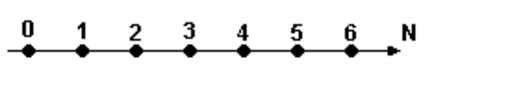
\includegraphics[width=3.44in,height=0.58in]{capitulos/conjuntos_numericos/media/image2.pdf}
	\end{Center}
\end{figure}

~~

Os intervalos no conjunto dos números naturais são escritos usando os símbolos 

> maior 

< menor 

$\geq$ maior ou igual e

$\leq$ menor ou igual.

Vejamos os exemplos:

\begin{texemplo}
	
	Escreva os elementos do conjunto  A=$ \{ x \in \mathbb{N}  / x > 2 \} $  (Lê-se: x pertence aos Naturais, tal que x é maior do que 2) e represente-os em uma reta.

\textbf{Solução}: Escrevendo os elementos de A, temos: A= $ \{ 3,4,5,6,7,... \}$.

Mostrando esse conjunto na reta dos números naturais, colocamos pontos cheios pretos para os elementos do conjunto \textbf{A e vazios para os elementos que não pertencem ao conjunto A.}

\begin{figure}[H]
	\begin{Center}
		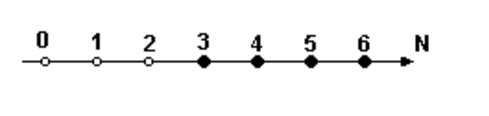
\includegraphics[width=3.26in,height=0.77in]{capitulos/conjuntos_numericos/media/image3.pdf}
	\end{Center}
\end{figure}

~~
\end{texemplo}

\begin{texemplo} 
	Escreva os elementos do conjunto~ B=$ \{ x \in \mathbb{N}  / 1< x <5 \} $  ( Lê-se: x pertence aos Naturais, tal que x é maior do que 1 e menor do que 5. (ou, x pertence aos Naturais , tal que 1 é menor do que x e x é menor do que 5) e represente-os em uma reta.

\textbf{Solução:} Usando a mesma representação do Exemplo 2.1, temos: B=$ \{ 2,3,4 \} $. Mostrando esse conjunto na reta dos números naturais, temos:

\begin{figure}[H]
	\begin{Center}
		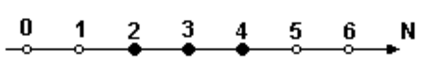
\includegraphics[width=2.93in,height=0.45in]{capitulos/conjuntos_numericos/media/image4.pdf}
	\end{Center}
\end{figure}
\end{texemplo}

\begin{texemplo}
Escreva os elementos do conjunto C, representado na reta numerada:

\begin{figure}[H]
	\begin{Center}
		
\includegraphics[width=4.17in,height=0.51in]{capitulos/conjuntos_numericos/media/image5.pdf}
	\end{Center}
\end{figure}

\textbf{Solução:}\quad Podemos escrever os elementos desse conjunto de duas maneiras: por extensão (descrevendo um a um) 

$$ C=\{5,6,7,8,9,10,\dots\}$$

\quad ou usando os símbolos de desigualdade  

\quad $C= \{ x \in \mathbb{N} / x  5 \}$ ou ainda $C= \{ x \in \mathbb{N} / x > 4 \}$ \qedsymbol{}
\end{texemplo}

\begin{exercicios}
    \exitem{} Escreva por extensão os elementos dos conjuntos:
    \begin{multicols}{2}
        a) A=$ \{x \in \mathbb{N} / x > 5 \}$ 

        b) B=$ \{ x \in \mathbb{N} / 1 < x < 10 \}$ 

        c) C=$ \{ x \in \mathbb{N} / x \leq 6 \} $
        
        d) D=$ \{ x \in \mathbb{N} / 2 \leq x < 8 \} $
        
        e) E=$ \{x \in \mathbb{N} / 2 < x \leq 5 \}$
        
        f) F=$ \{x \in \mathbb{N} / 2 > x \textrm{ ou } x > 5 \}$
    \end{multicols}
	\exitem{} Represente os conjuntos do Ex.1 graficamente.

	\exitem{} Verifique se as quantidades das grandezas abaixo podem ser expressas com números naturais:

        a) População de uma cidade.

        b) Número de porcos criados em uma granja por ano.

        c) A velocidade de uma pessoa em uma corrida de maratona.

        d) O número de escovas de dentes produzido mensalmente por uma indústria.

        e) A taxa de variação da cesta básica em um estado do Brasil em um determinado mês.

	\exitem{} As notas das provas escolares são expressas em números naturais?

	\exitem{} Existe um número \textbf{natural} X que somado com 5 dê 3? (ou seja: 5 + X = 3)

	\exitem{} Verifique se as operações abaixo geram números naturais:
    \begin{multicols}{2}
        a) 5 + 8 = 

        b) 3 – 5 =
        
        c) 5$\cdot$ 8
        
        d) 8 $\div$ 5 =
    \end{multicols}
\end{exercicios}

\section{Conjunto dos Números Inteiros Relativos ($\mathbb{Z}$)}

As letras (b) e (d) do Exercício 1.1.6 ilustram problemas de operações com números naturais cuja solução gera números não naturais. Portanto, é necessário admitir a existência de outros tipos de números.

Se as quantidades ou grandezas inteiras mudam seu significado de acordo com um referencial, pode-se representa-las usando um sinal e um número. Vejamos alguns exemplos:

\textbf{Saldo bancário:} se temos dinheiro depositado, dizemos que o saldo é positivo. Se gastamos mais dinheiro do que temos e o banco nos empresta, dizemos que o saldo é negativo. Assim, se o saldo é +3.500,00 reais, significa que temos esse montante na conta. A referência, é o saldo zero. Neste caso, não temos nada, mas também não devemos ao banco.

\textbf{Temperatura:} a temperatura é uma grandeza associada ao estado térmico de um corpo: Quanto mais calor o corpo possui, maior será a temperatura e quanto mais frio, menor. Pela escala Celsius, a referência é a temperatura da água congelada: 0 \textsuperscript{o}C. Assim, na madrugada de um dia de inverno podemos ter temperaturas negativas, como -5\textsuperscript{o}C e ao meio-dia, positivas, como + 15\textsuperscript{o}C.

\textbf{Taxas de variações:} as variações de cotação de moedas, como o dólar, por exemplo, são dadas usando a referência zero, ou seja quando não varia. Assim, +2  significa que o dólar 'caiu'. Essas taxas de variações são muito usadas na economia: na bolsa de valores para indicar a tendência das ações; nas análises de desempenho de empresas (crescimento/decrescimento). Na física, o sinal da velocidade de um corpo indica o sentido do deslocamento.

Os números inteiros relativos podem ser representados da seguinte forma: 

 $$(\mathbb{Z})  = \{\dots,-6,-5,-4-3,-2,-1,0,+1,+2,+3,+4,+5,+6,\dots\}$$

A representação gráfica do conjunto  \(\mathbb{Z}\)  é:

\begin{figure}[H]
	\begin{Center}
		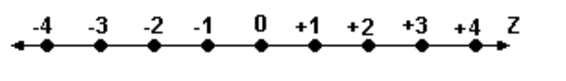
\includegraphics[width=3.77in,height=0.54in]{capitulos/conjuntos_numericos/media/image6.pdf}
	\end{Center}
\end{figure}

~~

Escrevendo o conjunto $\mathbb{Z}$  usando símbolos, temos: 

$\mathbb{Z} = \{x \in \mathbb{Z}/ -\infty < x < +\infty\}$.

\subsection{Operações em $\mathbb{Z}$}

\subsubsection{Adição e subtração de números inteiros}

Ao operar com números inteiros relativos, precisamos identificar inicialmente a operação solicitada e em seguida o sinal dos números.

\begin{figure}[H]
	\begin{Center}
		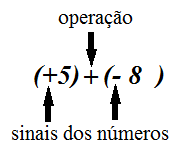
\includegraphics[width=1.88in,height=1.64in]{capitulos/conjuntos_numericos/media/image7.png}
	\end{Center}
\end{figure}

~~
\begin{center}
\textbf{Regra da adição de dois números inteiros}:
\end{center}

\begin{caixa}
    sinais iguais $\Rightarrow$ adiciona e usa o mesmo sinal no resultado

    sinais diferentes $\Rightarrow$ subtrai e usa o sinal do maior no resultado

\end{caixa}
\textbf{Exemplos:}
\begin{multicols}{2}
    1)$(+5) + (+3) = +5+3 = +8$ 

    2)$(+5) + (- 3) = +5 - 3 = +2$ 
    
    3)$(-5) + (+ 3) = -5 + 3 = -2$

    4)$(-5) + (- 3) = -5 - 3 = -8$
\end{multicols}
\subsubsection{Multiplicação e divisão de números inteiros}
 
\begin{center}
    \textbf{Regra da Subtração de dois números inteiros}
\end{center}
\begin{caixa}
Troca o sinal do segundo número e usa a regra da adição.
\end{caixa}
\textbf{Exemplos:}
\begin{multicols}{2}
1)$(+5) - (+ 3) = (+5) + (- 3) = +2$

2)$(+5) - (- 3) = (+5) + (+ 3) = +8$

3)$(-5) - (- 3) = (-5) + (+ 3) = - 2$

4)$(-5) - (+ 3) = (-5) + (- 3) = - 8$
\end{multicols}
\begin{center}
\textbf{Regra da Multiplicação e Divisão: }(para o sinal do resultado)
\end{center}
\begin{caixa}
sinais iguais $\Rightarrow$resultado positivo

sinais diferentes $\Rightarrow$resultado negativo
\end{caixa}

\textbf{Exemplos:}

\begin{multicols}{2}
	1)$(+5) \cdot (+4) = +20$

    2)$(+20) : (-4) = - 5$
    
    3)$ (+20) : (+4) = + 5$
    
    4)$(+5) \cdot (-4) = - 20$
\end{multicols}

\subsubsection{Potênciação de números inteiros}
 
\begin{caixa}
    \begin{tdefinicao}
    A potência~ \textit{b\textsuperscript{n}}~ , para  o expoente \textit{n $ \in $   \( \mathbb{N} \) } e a base \textit{b $ \in $   \( \mathbb{Z} \) ~ ,} é o produto de \textit{b}, \textit{n} vezes,  por ele mesmo:

    \begin{figure}[H]
	    \begin{Center}
		    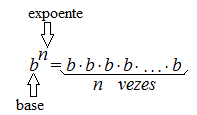
\includegraphics[width=2.05in,height=1.2in]{capitulos/conjuntos_numericos/media/image8.png}
	    \end{Center}
    \end{figure}
    \end{tdefinicao}
\end{caixa}

\textbf{Exemplos: }
Calcule (a) $2^4$, (b) $(-3)^3$, (c) $(-2)^4$ e (d) $-2^4$

\textbf{Solução}: 
\begin{enumerate}[label=\alph*]
    \item \textit{2\textsuperscript{4}}~=~2 $ \cdot $  2 $ \cdot $  2  $ \cdot $  2  = \textit{16}

    \item (-3)\textit{\textsuperscript{3}~ = (-3)} $ \cdot $  \textit{(-3)} $ \cdot $  \textit{(-3)} = \textit{-27}

    \item \textit{(-2)\textsuperscript{4} = (-2)} $ \cdot $  \textit{(-2)} $ \cdot $  \textit{(-2)} $ \cdot $  \textit{(-2)=~16  }

    \item -2\textit{\textsuperscript{4}~ = -2 }$ \cdot $  \textit{2} $ \cdot $  \textit{2} $ \cdot $ \textit{2 = -16}
\end{enumerate}

\textbf{Observemos que:}
\begin{caixa}
\begin{enumerate}
	\item Se a base é positiva (\textit{b > 0}) então \textit{b\textsuperscript{n}} > 0.

	\item Se a base é negativa (\textit{b < 0}) e :

    \quad Se \textit{n é par então b\textsuperscript{n} > 0}

    \quad Se \textit{n é ímpar então b\textsuperscript{n} < 0.}

	\item Se a base é 1 (\textit{b = 1}) então \textit{b\textsuperscript{n}} \textit{= 1}, para qualquer \textit{n $ \in $   \( \mathbb{N} \) .} 
\end{enumerate}
\end{caixa}

\subsubsection{Radiciação de números inteiros}
 
\begin{caixa}
    \begin{tdefinicao}
        A raiz \textit{n-ézima, }para\textit{ n }  \(\in \mathbb{\mathbb{N}} \)  , de um número \textit{b}   \(\in \mathbb{Z} \) é \textit{x}   \(\in \mathbb{Z} \)  se e somente se \textit{x\textsuperscript{n} = b}.
        \[ \sqrt[n]{b}=x \Longleftrightarrow   x^{n}=b. \]
    \end{tdefinicao}
\end{caixa}

\textbf{Exemplos}:

\begin{enumerate}
	\item  \( \sqrt[3]{8}=2~~ \Longleftrightarrow   2^{3}=8. \) 

	\item  \( \sqrt[3]{ \left( -8 \right) }=-2~~ \Longleftrightarrow    \left( -2 \right) ^{3}=-8. \) 

	\item  \( \sqrt[]{10}~~ \) não é um número inteiro, pois \textit{3\textsuperscript{2} < 10 < 4\textsuperscript{2}}.

	\item  \( \sqrt[]{4}=-2~~ \Longleftrightarrow    \left( -2 \right) ^{2}=4 \) ,~mas também   \( \sqrt[]{4}=2~~ \Longleftrightarrow    \left( 2 \right) ^{2}=4 \) . 
\end{enumerate}

Então~  \( \sqrt[]{4}= \pm ~2   \) \qedsymbol{}

\begin{exercicios}

	\exitem{} Resolva as expressões numéricas:
    \begin{multicols}{2}
        a)$(+15)+(-12) =$
        
        b)$(-15)+(-10) =$

        c)$(+8)+(-12)-(+5) =$
        
        d)$(-7)-(-9)-(+3) =$

        e)$(+6) : (-3) =$
        
        f)$(-7) \cdot (-5) =$

        g)$1- (-3)+(-4)=$
        
        h)$-4-[3+5(5 - 2)]=$

        i)$3\cdot(5 - 8)-(8 - 3)+6 =$
        
        j)$-[-4 -3\cdot(7-4)-(2-5)]=$
    \end{multicols}
	\exitem{} O saldo bancário de um correntista no dia 1\textsuperscript{o }do mês era de R$\$$  3.500,00 e no dia 3, entrou um cheque para ser descontado de R$\$$  4.350,00. Qual é o saldo no dia 3 ?

	\exitem{} Expresse e resolva as seguintes situações, usando números relativos:

    \quad a) Uma pessoa tem $50$ reais e \textbf{perde} $30$ reais.

    \quad b) Uma pessoa tem $100$ reais e \textbf{paga} uma dívida $40$.

    \quad c) Uma pessoa tem uma \textbf{dívida} de $100$ reais e \textbf{ganha} $50$ reais.

    \quad d) Uma pessoa tem uma \textbf{dívida} de $200$ reais e \textbf{perde} $70$ reais.

	\exitem{} Em um dia de inverno a temperatura máxima foi de \textit{18\textsuperscript{o}C} e a mínima de \textit{-3\textsuperscript{o}C}. Qual foi a variação de temperatura?

	\exitem{} Uma peça de metal estava a 80\textsuperscript{o}C e foi resfriada variando sua temperatura em 90\textsuperscript{o}C. Qual é a temperatura final da peça?

	\exitem{} Considere o nível do mar como altitude \textit{0 m}, acima positiva e abaixo negativa. Se a cidade \textbf{A} está a \textit{+ 450 m} e a \textbf{B} está a \textit{+230 m}, qual é a diferença de altitude entre as cidades?

	\exitem{} Existe um número \textbf{inteiro} $X$ que somado com 5 dê 3? (ou seja: 5 + X = 3)

	\exitem{} A divisão~ 6/2~~é  número \textbf{inteiro} ? e a divisão 6/4 ?

	\exitem{} Resolva as potências:
	\begin{multicols}{4}
		a) $4^2$
	
		b) $(-4)^3$
	
		c) $0^5$

		d) $1^100$
	
		e) $ -5^{2}$
	
		f) $-2^{4}$

		g) $-2^{4}$

		h)  $-2^{5}$
	\end{multicols}

	\exitem{} Resolva as raízes:
	\begin{multicols}{3}
		a)  \( \sqrt[]{9} \)

		b)  \( \sqrt[3]{27} \)
		
		c)  \( \sqrt[3]{-27} \)
		
		d)  \( \sqrt[4]{16} \)
		
		e)  \( \sqrt[6]{64} \)
		
		f)  \( \sqrt[5]{32} \)
		
		g)  \( \sqrt[5]{-32} \)
		
		h)  \( \sqrt[3]{-64} \)
	\end{multicols}
\end{exercicios}

\section{Conjunto dos Números Racionais ( \( \mathbb{Q} \) )}

Os números racionais são aqueles que podem ser escritos na forma de fração  \( \frac{a}{b} \) , onde \textit{a} e \textit{b} são números inteiros, com \textit{b} diferente de zero. Simbolizamos o conjunto dos racionais com a letra $\mathbb{Q}$. Escrevendo em linguagem matemática:

 $ \mathbb{Q}  =  \{ x \in \mathbb{Q}$ se $x = a/b \} $  para $a$ e $b \in \mathbb{Z} $  e $b \neq 0$.

Assim, qualquer fração é um número racional, por exemplo  \( \frac{1}{2} \)  ;  \( \frac{5}{4} \)  ; \( -\frac{3}{5} \) ; ...

Da mesma forma, qualquer número inteiro é também um número racional, pois podemos escrevê-lo em forma de fração. Por exemplo:

 \( 2=\frac{4}{2}=\frac{10}{5} \) ;~~~~~~~~~~~~~  \( -5=\frac{-10}{2}=\frac{30}{-6}=-\frac{15}{3} \) .

\textbf{Equivalência de frações}: uma fração  \( \frac{a}{b} \)   não se altera se multiplicamos ou dividimos o numerador e o denominador pelo mesmo número \textit{m}, desde que\textit{ m $ \neq $  0 }e\textit{ m  \(\in \mathbb{Z} \) }.

 \quad \quad {\fontsize{14pt}{16.8pt}\selectfont   \( \frac{a}{b}=\frac{a \cdot m}{b \cdot m} \) ~~~~~~ ou~~~~~~  \( \frac{a}{b}=\frac{\text{a~ : m}}{\text{b~ : m}} \)  }

Observe-se que para a divisão, \textit{a} e \textit{b} devem ser divisíveis por \textit{m}. Com essa propriedade podemos transformar uma fração em outra equivalente, porém com denominador diferente. Vejamos os exemplos:

\textbf{Exemplos:}

\begin{enumerate}
	\item  \( \frac{1}{2}=\frac{2}{4} \)  . Nesse caso, a primeira fração foi multiplicada por \textit{m=2}.

	\item   \( \frac{12}{8}=\frac{3}{2} \). Esse caso é conhecido como simplificação de frações. Dividimos o numerador e o denominador por \textit{m=4.}

	\item Para~transformar   \( \frac{3}{4} \) ~ em uma fração com denominador igual 16, podemos usar \textit{m=4}.~Assim~   \( \frac{3}{4}=\frac{12}{16} \) ~ são equivalentes.
\end{enumerate}

\subsection{Adição e subtração de frações }

\quad O sinal do resultado da adição e subtração de frações segue as regras operatórias dos números inteiros e das operações com frações.

\quad 
\subsubsection{Frações com denominadores iguais}

Sejam \textit{a, b} e \textit{c} números inteiros: 

\textbf{\quad ~~~~  \( \frac{a}{b}+\frac{c}{b}=\frac{a+c}{b} \) \quad }{\fontsize{16pt}{19.2pt}\selectfont \quad , para \textit{b ~  \( \mathbb{Z} \)  $ \neq $  0}.}

\textbf{Exemplos: }

\begin{enumerate}
	\item  \( \frac{1}{4}+\frac{5}{4}=\frac{1+5}{4}=\frac{6}{4}=\frac{3}{2} \) \quad \quad b)  \( \frac{3}{5}-\frac{4}{5}=\frac{3-4}{5}=\frac{-1}{5}=-\frac{1}{5} \) \quad 
\end{enumerate}

\subsubsection{Frações com denominadores diferentes}

Se os denominadores das frações são diferentes, transformamos as frações de tal forma que os denominadores sejam iguais. Usar o menor múltiplo comum (MMC) dos denominadores das frações dadas como denominador das novas frações é uma estratégia bem eficiente. Ou de modo geral, 

\quad  \( \frac{a}{b}+\frac{c}{d}=\frac{ad+cb}{bd}~~~ \) {\fontsize{16pt}{19.2pt}\selectfont  , para \textit{b }e\textit{ d  ~  \( \mathbb{Z} \)   $ \neq $  0} \qedsymbol{}}

\textbf{Exemplos:}

\begin{enumerate}
	\item  \( \frac{1}{4}+\frac{3}{2}=\frac{1+6}{4}=\frac{7}{4} \) \quad \quad \quad 2){\fontsize{16pt}{19.2pt}\selectfont   \( \frac{1}{4}-\frac{2}{3}=\frac{3-8}{12}=-\frac{5}{12} \) }
\end{enumerate}

\subsection{Multiplicação de frações:}

Sejam \textit{a, b,c} e \textit{d} números inteiros: 

\begin{caixa}
\textbf{Multiplica-se numerador com numerador e denominador com denominador. }

$$ \frac{a}{b} \cdot \frac{c}{d}=\frac{a \cdot c }{b \cdot d}\textrm{,  para }$$ b $$\textrm{ e } d \in \mathbb{Z} \neq 0 \textrm{.}$$
\end{caixa}
\textbf{Exemplos:}

\begin{enumerate}
	\item  \( \frac{1}{4} \cdot \frac{3}{2}=\frac{3}{8} \) \quad \quad \quad 2){\fontsize{16pt}{19.2pt}\selectfont   \( \frac{1}{4} \cdot  \left( -\frac{2}{3} \right) =-\frac{2}{12}=-\frac{1}{6} \) }
\end{enumerate}

\textbf{Propriedade do cancelamento:}

Algumas multiplicações podem ser simplificadas, diminuindo os números a serem operados.

\textbf{Exemplos: }

1) Resolva \( \frac{12}{5} \cdot \frac{3}{2}\text{~~~ .} \) 

Simplificando o \textit{12} com o \textit{2}, por \textit{2,} obtemos   \( \frac{6}{5} \cdot \frac{3}{1}=\frac{18}{5} \) {\fontsize{16pt}{19.2pt}\selectfont .}

2) Resolva \( \frac{18}{15} \cdot \frac{5}{2} \cdot \frac{9}{2}\text{.} \)

A utilização da regra da multiplicação diretamente, neste caso, gera operações com números relativamente grandes. Utilizando o cancelamento, essa dificuldade é remediada.

Simplificando o \textit{18} com \textit{2} e o \textit{15} com o \textit{5}, obtemos  \( \frac{9}{3} \cdot \frac{1}{1} \cdot \frac{9}{2}. \) 

Simplificando o \textit{3} com o \textit{9}, obtemos  \( \frac{3}{1} \cdot \frac{1}{1} \cdot \frac{9}{2}=\frac{27}{2}~. \) \quad 

\subsection{Divisão de frações}

\begin{caixa}
\quad Inverte-se a segunda fração e multiplica-se pela primeira.
~ \quad \quad  \( \frac{a}{b}:\frac{c}{d}=\frac{a}{b} \cdot \frac{d}{c}=\frac{ad}{bc}~~ \) ~ , para \textit{b} e \textit{d} \textit{~  \( \in \mathbb{Z} \) }  $ \neq $   0.
\end{caixa}
A regra dos sinais é idêntica à regra da divisão dos números inteiros.

\textbf{Demonstração: }

Seja \( \frac{a}{b}~:~\frac{c}{d}=N \) , sendo $\mathbb{N}$  \( \in \mathbb{Q} \).

Escrevendo \( \frac{a}{b}~:~\frac{c}{d}=N \) ~ como  \( ~~\frac{~\frac{a}{b}}{\frac{c}{d}}~ =N \)  , pode-se multiplicar ambos os membros dessa equação por \textit{d/c}.

\quad  \(\frac{~\frac{a}{b}}{\frac{c}{d}}  \cdot  \frac{c}{d} =N  \cdot  \frac{c}{d} \) 

Cancelando o denominador \textit{c/d}~ com o fator \textit{c/d}~ do primeiro membro, tem-se:

\quad  \( ~\frac{a}{b}~ =N  \cdot  \frac{c}{d} \) 

Para isolar \textit{N}, multiplica-se ambos os membros dessa equação por \textit{d/c}. Tem-se:

\quad  \( \frac{a}{b} \cdot  \frac{d}{c}~ =N  \cdot  \frac{c}{d} \cdot  \frac{d}{c}=N \) 

O produto das frações do lado direito é 1. Portanto, tem-se:

\quad  \( N=\frac{a}{b}~:~\frac{c}{d}= \frac{a}{b} \cdot  \frac{d}{c} =\frac{ad}{bc}~ \) ~~~ \qedsymbol{}\quad 

\textbf{Exemplos:}

\begin{enumerate}
	\item  \( \frac{3}{4}:\frac{1}{2}=\frac{3}{4} \cdot \frac{2}{1}=\frac{3}{2} \) \quad \quad 2)\(  \left( -\frac{1}{3} \right) : \left( -\frac{2}{5} \right) = \left( -\frac{1}{3} \right)  \cdot  \left( -\frac{5}{2} \right) =+\frac{5}{6} \)
\end{enumerate}

\subsection{Números decimais e frações }

Os \textit{números decimais finitos} podem ser representados na forma de frações decimais, usando a propriedade da equivalência de frações. Portanto, são números racionais. Veja os exemplos:

\textbf{Exemplos:}

1)  \( 0,3=0,3 \cdot \frac{10}{10}=\frac{3}{10}~~ \) \quad \quad \quad \quad 

2)  \( 0,25=0,25 \cdot \frac{100}{100}=\frac{25}{100}~~ \)  \quad \quad \quad \quad 

3)  \( 1,302=1,302 \cdot \frac{1000}{1000}=\frac{1302}{1000}~~ \) ~~~~ 

Generalizando a ideia apresentada nestes exemplos, podemos afirmar que para representar um número decimal finito na forma de fração

\begin{caixa}
\begin{Center}
Escrevemos o número sem a vírgula sobre \textit{10$ \cdot $ n}, sendo \textit{n} o número de casas depois da vírgula do número decimal.
\end{Center}
\end{caixa}

Os números \textit{decimais periódicos infinitos} também podem ser representados na forma de frações. Veja os exemplos:

\begin{texemplo}
Represente a dízima periódica 0,33333.... na forma de fração.

\textbf{Solução: }Vamos chamar esse número de \textit{r}:

\quad \textit{r = 0,333333....} . Multiplicando a equação toda por \textit{10}, porque o período tem somente um algarismo, temos:

\quad \textit{10r = 3,33333....} . Re-escrevendo o lado direito da igualdade, temos:

\quad \textit{10r = 3 + 0,33333.... = 3 + r} .~~ Adicionando (-r) nos dois lados da equação, temos:

\quad \textit{10r – r = 3}

\quad \textit{9r = 3}

\quad  \( r=\frac{3}{9}=\frac{1}{3}~~ \) \textit{, }portanto 1/3 é um número racional\textit{ \qedsymbol{}}

\end{texemplo}

\begin{texemplo}
Represente a dízima periódica \textit{r = 0,12121212....} na forma de fração.

\textbf{Solução: }Multiplicando a equação toda por \textit{100}, porque o período tem dois algarismos, temos:

\quad \textit{100 r = 12,121212 $ \ldots $ } . Re-escrevendo o lado direito da igualdade, temos:\quad 

\quad \textit{100 r = 12 + 0,12121212... = 12 + r}.~ Adicionando (\textit{-r}) nos dois lados da equação, temos:

\quad \textit{100r – r = 12}

\textit{\quad 99r = 12}

\quad  \( r=\frac{12}{99}~~~ \) \textit{~~~ ,} portanto 12/99 é um número racional\textit{\qedsymbol{}}
\end{texemplo}
\quad Regra para escrever dízimas periódicas, menores do que 1, na forma de fração:

\begin{caixa}

\textbf{1º~  Escreve-se os algarismos do período no numerador;}

\textbf{2º~  Escreve-se o denominador com tantos noves, quantos forem os algarismos do período.}

\end{caixa}
\quad Com esta regra, podemos representar qualquer dízima periódica na forma de um número racional. Veja os exemplos e confira com sua calculadora:

\textbf{Exemplos:}

1)  \( 0,2222 \ldots =\frac{2}{9} \)  \quad \quad 2)  \( 0,252525 \ldots =\frac{25}{99} \) \quad \quad 3)~  \( 0,245245245 \ldots =\frac{245}{999} \) 

\begin{exercicios}

	\exitem{} Resolva as adições e subtrações com as frações:

a)\textbf{  \(  \left( -\frac{1}{3} \right) + \left( -\frac{2}{3} \right) = \) \quad \quad \quad }d){\fontsize{16pt}{19.2pt}\selectfont   \( -\frac{2}{7}-\frac{3}{14}+\frac{3}{2}= \) }

b){\fontsize{16pt}{19.2pt}\selectfont   \(  \left( -\frac{4}{3} \right) - \left( -\frac{2}{5} \right) + \left( -\frac{1}{6} \right) = \) \quad e)  \( -\frac{5}{6}+\frac{3}{8}+\frac{1}{2}= \) }

c)  \( 1+\frac{3}{10}-\frac{12}{15}= \) \quad \quad \quad f){\fontsize{16pt}{19.2pt}\selectfont   \( ~\frac{5}{2}-2+\frac{2}{4}= \) }

	\exitem{} Resolva as operações com as expressões fracionárias:

a)\textbf{  \( \frac{1}{2}- \left( \frac{1}{3}+\frac{2}{3} \right) =~  \) \quad \quad \quad }d)\textbf{  \( -3 \cdot  \left( -\frac{1}{3}+\frac{2}{5} \right) =~  \) \quad }

b)~  \( -\frac{1}{3} \cdot  \left( -2+\frac{2}{3} \right) =~  \) ~~~~~~~ \quad \quad e)~  \( -5: \left( \frac{1}{2}-\frac{2}{3} \right) =~~  \) 

c)  \( -6 \cdot  \left( \frac{1}{3}+\frac{3}{4} \right) =~  \) \quad \quad \quad f)~~  \( -3 \cdot  \left( -\frac{1}{3} \right) +\frac{3}{4}:\frac{3}{2}=~  \) ~~~~~~~ 
\end{exercicios}

\section{Conjunto dos números reais ($\mathbb{R}$)}

Os recursos utilizados para escrever uma dízima periódica na forma de fração, tem por base o fato de existir um período (números que se repetem). Existem muitos números decimais não periódicos. Vejamos alguns exemplos:

$ \pi = 3,1415926$... Conhecido como número pi. Está presente em vários problemas de geometria.

$e = 2,7182818284590452353602874$... Conhecido como número de Euler, ou número e.

 \( \sqrt[]{2}=1,414214 \ldots  \)  É uma raiz não exata. As raízes não exatas não são dízimas periódicas.

$\varnothing =1,6180339887$... ou ~  \(  \varnothing =\frac{1+\sqrt[]{5}}{2} \) ~ é conhecido como o número de ouro, amplamente usado por arquitetos gregos para projetar construções e por artistas para determinar proporções em desenhos do corpo humano. 

A esses números, que é impossível escreve-los na forma de fração, damos o nome de números irracionais. Além de números especiais como o pi, o número de Euler e o número de ouro, as raízes não exatas são exemplos mais comuns de números irracionais. O uso das propriedades e operações com raízes não exatas (radicais) são frequentes em aplicações na ciência.
\begin{caixa}
	\begin{tdefinicao}
		
		O conjunto dos Números Reais é a união do conjunto dos Racionais e dos Irracionais.

		\quad  \( R \)  =  \( \mathbb{Q} \cup \mathbb{I}\) \qedsymbol{}
	\end{tdefinicao}
\end{caixa}
A representação do conjunto  \( R \)  na reta numérica é uma reta cheia (reta real).

\begin{figure}[H]
	\begin{Center}
		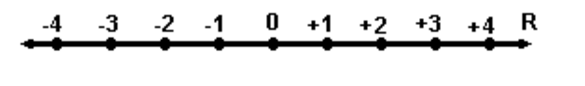
\includegraphics[width=3.9in,height=0.57in]{capitulos/conjuntos_numericos/media/image9.pdf}
	\end{Center}
\end{figure}

~~

Veja alguns exemplos de intervalos em  \( \mathbb{R} \) e suas respectivas representações na reta numerada:

\begin{figure}[H]
	\begin{Center}
		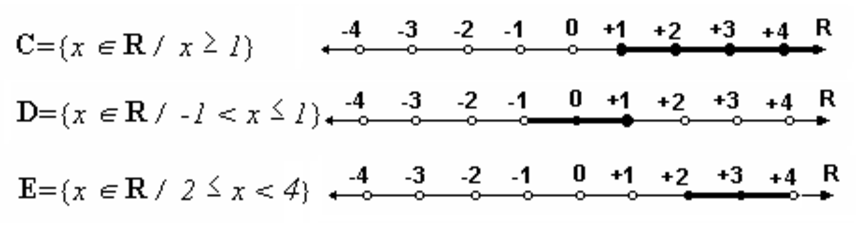
\includegraphics[width=5.72in,height=1.53in]{capitulos/conjuntos_numericos/media/image10.pdf}
	\end{Center}
\end{figure}

~~

Os conjuntos também podem ser representados usando parêntesis para \textit{intervalos abertos, por exemplo:}

(a,b) significa $ \{ $ \textit{ x \( \in \mathbb{R} \)  / a < x < b$ \} $ }

e com colchetes para \textit{intervalos fechados, por exemplo:}

[a,b] significa =$ \{ $ \textit{ x \( \in \mathbb{R} \)  / a$\leq$  x $\leq$  b$ \} $ .}

\begin{caixa}
	\begin{tdefinicao}

	Seja \textit{b um número real,~ m e n~números inteiros positivos.  Então,}

	\quad   \( b^{\frac{m}{n}}=\sqrt[n]{b^{m}} \) {\fontsize{14pt}{16.8pt}\selectfont .}
	\end{tdefinicao}
\end{caixa}
\textbf{Exemplo: \( ~~\sqrt[3]{3^{2}}=3^{\frac{2}{3}} \) ~ \qedsymbol{}}

\subsection{Propriedades dos radicais}

Sejam \textit{a e b números reais; m,n e p números inteiros positivos maiores do que 1.}

\textbf{P1)  \( \sqrt[n]{a \cdot b}=\sqrt[n]{a} \cdot \sqrt[n]{b} \) }

\textbf{P2)  \( \sqrt[n]{\frac{a}{b}}=\frac{\sqrt[n]{a}}{\sqrt[n]{b}} \) ~~para  \textit{b $ \neq $ ~ 0.}}

\textbf{P3)  \( \sqrt[n]{\sqrt[m]{b}}=\sqrt[nm]{b} \) }

\textbf{P4)  \(  \left( \sqrt[n]{b^{m}} \right) ^{p}=\sqrt[n]{a^{mp}} \) }

\textbf{P5) Para b $ \geq $ ~0    \( \sqrt[n]{b^{n}}=b . \) }

\textbf{P6)~Para~b~<~0       \( \sqrt[n]{b^{n}}= \left\{ \begin{matrix}
 \vert b \vert \textrm{ se n é par}\\
-b \textrm{ se n é ímpar} \\
\end{matrix} \right\}
 ~ \) }

\textbf{Exemplos: Simplifique os radicais:}

\begin{enumerate}
	\item  \( \sqrt[3]{81} \)  . Para simplificar esse radical vamos utilizar as propriedades P1 e P5.

 \[ \sqrt[3]{81}=\sqrt[3]{3^{4}}=\sqrt[3]{3^{3} \cdot 3}=3 \cdot \sqrt[3]{3} \] 

	\item  \( \sqrt[]{27y^{9}} \) ~~ se y > 0. Para simplificar esse radical vamos utilizar as propriedades P1 e P5.
\end{enumerate}

\quad  \( \sqrt[]{27y^{9}}=\sqrt[]{3  \cdot 3^{2} \cdot y^{8} \cdot y}=3y^{4}\sqrt[]{\text{3 y}} \) ~ \qedsymbol{}

\subsection{Racionalização de denominadores}

O denominador de algumas frações podem ter radicais. Nesse caso podemos usar a propriedade P5 para racionalizar (tornar racional) o denominador. 

\begin{texemplo}
	
Racionalize o denominador da fração~~   \( \frac{1}{\sqrt[]{3}}. \)

\textbf{Solução: Multiplicando-se a fração dada por 1, escrito na forma  \( \frac{\sqrt[]{3}}{\sqrt[]{3}}. \) ~~ não a alteramos. Então,  \( \frac{1}{\sqrt[]{3}} \cdot \frac{\sqrt[]{3}}{\sqrt[]{3}}=\frac{\sqrt[]{3}}{3} \) ~ \qedsymbol{}}
\end{texemplo}
\subsection{Operações com radicais}

\subsubsection{Adição e subtração}

Só é possível adicionar ou subtrair radicais semelhantes (\textit{índices e radicandos idênticos). }

\textbf{Exemplos:}

\begin{enumerate}
	\item  \( \sqrt[]{2}+3\sqrt[]{2}-5\sqrt[]{2}=-\sqrt[]{2} \) 

	\item  \( \sqrt[]{3}-2\sqrt[]{27}-\frac{\sqrt[]{12}}{2}.~ \)  Nesse caso, os radicais não são semelhantes. Porém,

 \( \sqrt[]{27}=3\sqrt[]{3} \) ~~e   \( \frac{\sqrt[]{12}}{2}=\frac{2\sqrt[]{3}}{2}=\sqrt[]{3} \) ~~ (usando as propriedades \textbf{P1 e P5). Substituindo estas igualdades na expressão dada, temos:}

 \( \sqrt[]{3}-3\sqrt[]{3}-\sqrt[]{3}=-3\sqrt[]{3}~ \) .
\end{enumerate}
	\subsubsection{Multiplicação e divisão de radicais}

As propriedades \textbf{P1 e P2 resolvem as operações de multiplicação e divisão, respectivamente, para radicais de mesmo índice. }

\textbf{Exemplos:}

\begin{enumerate}
	\item  \( \sqrt[]{2} \cdot \sqrt[]{5}=\sqrt[]{10} \) ~ . Foi usada a propriedade P1.

	\item  \( \sqrt[]{6}\text{~ : }\sqrt[]{2}=\sqrt[]{3} \) ~~~ Foi usada a propriedade P2.

	\item  \( \sqrt[]{3} \cdot \sqrt[4]{2}= \) 

Como o MMC(2,4)=4,~vamos transformar os radicais equivalentes com índice  4 e usar a propriedade P1.

 \[ \sqrt[2 \cdot 2]{3^{1 \cdot 2}} \cdot \sqrt[4]{2}=\sqrt[4]{3^{2}} \cdot \sqrt[4]{2}=\sqrt[4]{18} \] 

	\item  \( \sqrt[4]{2} \cdot \sqrt[6]{3}= \) 

Como o MMC(4,6)=12,~vamos transformar os radicais equivalentes com índice  12 e usar a propriedade P1.

 \[ \sqrt[4 \cdot 3]{2^{1 \cdot 3}} \cdot \sqrt[6 \cdot 2]{3^{1 \cdot 2}}=\sqrt[12]{8} \cdot \sqrt[12]{9}=\sqrt[12]{72} \] 

	\item  \( \sqrt[4]{2} \cdot \sqrt[6]{2}= \) 
\end{enumerate}

Como o MMC(4,6)=12,~vamos transformar os radicais equivalentes com índice  12 e usar a propriedade P1..

 \[ \sqrt[4 \cdot 3]{2^{1 \cdot 3}} \cdot \sqrt[6 \cdot 2]{2^{1 \cdot 2}}=\sqrt[12]{2^{5}}= \] 

Nesse caso (bases dos radicandos iguais) poderíamos usar a Def. 1.4.2 e resolver como multiplicação de potências de mesmas bases.

 \( \sqrt[4]{2} \cdot \sqrt[6]{2}=2^{\frac{1}{4}} \cdot 2^{\frac{1}{6}}=2^{\frac{5}{12}}=\sqrt[12]{2^{5}}~~~~~ \) \qedsymbol{}

\begin{exercicios}
	
	\exitem{} Calcule as raízes:

\begin{multicols}{6}
	
	a) \( \sqrt[3]{27} \)
	
	b)  \( \sqrt[3]{\frac{8}{27}} \)
	
	c)  \( \sqrt[3]{64} \)
	
	d)  \( \sqrt[5]{32} \)
	
	e)  \( \frac{\sqrt[]{64}}{\sqrt[4]{16}} \)
	
	f)  \( \sqrt[4]{\frac{625}{81}} \) 
\end{multicols}

	\exitem{} Os radicais do Ex.5.1 são números racionais ou irracionais?

	\exitem{} Simplifique os radicais:
	\begin{multicols}{6}

		 a) \(\sqrt[]{8} \)
		 
		 b)  \( \sqrt[]{12} \)
		 
		 c)  \( \sqrt[3]{24} \)
		 
		 d)  \( \sqrt[4]{32} \) 
		 
		 e)  \( \sqrt[]{\frac{12}{45}} \)
		 
		 f)  \( \sqrt[3]{\frac{16}{125}} \)
	\end{multicols}
	\exitem{} Os radicais do Ex 5.3 são números racionais ou irracionais?

	\exitem{} Coloque os coeficientes no radicando:
	\begin{multicols}{6}

	a) \( 2 \sqrt[]{3} \)
	
	b)  \( 3 \sqrt[3]{2} \)
	
	c)  \( 7 \sqrt[]{2} \)
	
	d)  \( \frac{1}{2}\sqrt[3]{4} \)
	
	e)  \( 3~ \cdot   \sqrt[]{\frac{1}{2}} \)
	
	f)  \( 5~ \cdot   \sqrt[]{\frac{3}{4}} \) 
	\end{multicols}
	\exitem{} Resolva as operações com os radicais:
	\begin{multicols}{4}
		a)  \( 3 \sqrt[]{3}+5\sqrt[]{3}-\sqrt[]{3} \) 
		
		b)  \( \sqrt[]{\frac{1}{2}}-~3  \sqrt[]{\frac{1}{2}} \)
		
		c)  \( \sqrt[]{5}  \cdot  \sqrt[3]{2} \)
		
		d)  \( \sqrt[]{3}  \cdot  \sqrt[]{5} \cdot \sqrt[]{\frac{1}{2}} \)
		
		e)  \( \sqrt[3]{\frac{3}{4}} \cdot 3~ \sqrt[3]{\frac{1}{2}} \)
		
		f)  \( ~7 \sqrt[]{5}  \cdot  3 \sqrt[]{2} \)
		
		g)  \( \sqrt[]{10}~:~\sqrt[]{2} \)
		
		h)  \( \sqrt[]{10}\text{~ : }\sqrt[]{\frac{1}{2}} \) 
\end{multicols}
	\exitem{} Resolva os produtos:

\begin{multicols}{2}
	a) \( 2~ \left( \sqrt[]{5}+3\sqrt[]{5} \right)  \)
	
	b)  \( \sqrt[]{2}~ \left( \sqrt[]{3}+\sqrt[]{5} \right)  \)
	
	c)  \( \sqrt[]{6}~ \left( \sqrt[]{32}-\sqrt[]{3} \right)  \)
	
	d)  \(  \left( 2+\sqrt[]{2} \right)  \cdot  \left( 2-\sqrt[]{2} \right)  \)
	
	e)~  \(  \left( 3-\sqrt[]{5} \right) ^{2} \)
	
	f)  \(  \left( \sqrt[]{7}-2\sqrt[]{3} \right)  \cdot  \left( \sqrt[]{7}+2\sqrt[]{3} \right)  \)
\end{multicols}

	\exitem{} Racionalize os denominadores:

\begin{multicols}{5}

	a) \( \frac{1}{\sqrt[]{3}} \)
	
	b)  \( \frac{3}{\sqrt[]{2}} \)
	
	c)  \( \frac{7}{\sqrt[]{5}} \)
	
	d)  \( \frac{3}{2+\sqrt[]{3}} \)
	
	e)  \( \frac{1}{\sqrt[]{2}-\sqrt[]{3}} \)
	
	f)  \( \frac{35}{\sqrt[]{3}-5} \)
\end{multicols}

\exitem{} Verifique~se~~~   \( \frac{-3}{2}=\frac{3}{-2}=-\frac{3}{2~} \) .

\exitem{} Escreva o respectivo conjunto numérico a que pertence cada um dos seguintes números:  0; $-$ 1; $-$ 34;  \( \sqrt[3]{8} \) ; 0,454545...; 212; $-$ 46;  \( \sqrt[3]{2} \) ; 12,1829421; 2,99999... e 3,76.

\exitem{} Explique porque \textit{-5 é um número inteiro e também é um número racional.}

\exitem{} Explique porque \textit{$-$ 15 é um número racional e também é um número inteiro.}

\exitem{} Escreva os números abaixo em forma de fração:
\begin{multicols}{3}
	
a) \textit{0,3}=

b) \textit{0,55555.}..=

c) \textit{1,32}= 

d) \textit{0,212121}...=

e) \textit{1,3333..}.=

f) \textit{3,434343}...=
\end{multicols}

	\exitem{}  Explique porque \textit{0,77777...} é um número racional.

	\exitem{}  Explique porque ~ $ \pi $  = 3,1415927... é um número irracional.

	\exitem{}  Explique porque  \( \frac{4}{6}=\frac{2}{3} \)  ~~ 

	\exitem{}  Indique o conjunto de números adequado para cada variável:
	\begin{enumerate}[label=\alph*)]
    \item Tempo de vida de um pé de milho.

    \item Altura de um pé de soja.

    \item Número de vacas de uma propriedade.

    \item Produção leiteira.

    \item Teor de água do solo.

    \item Massa de solo.

    \item Massa de um suíno.

    \item Volume de água de uma amostra de solo.

    \item Número de frangos em um aviário.

    \item Diagonal de um quadrado.
\end{enumerate}
	\exitem{} Escreva os intervalos por compreensão:
	\begin{multicols}{2}
	
		a) \textbf{\textit{A}}\textit{=$ \{ $ 1,2,3,4,5$ \} $ }.
		
		b) \textbf{\textit{B}}\textit{=$ \{ $ -3,-2,-1,0,1,2$ \} $ }.

		c) os números reais maiores ou iguais a -3.
		
		d) os números reais entre -3 e 5.

		e) os números reais menores que 3 e maiores que 5.
	\end{multicols}

	\exitem{}  Represente os intervalos na reta real:
	\begin{multicols}{2}
	a) $P= \{ x \in {\mathbb{R} }/ -  1 < x < 3 \} $
	 
	b) $K= \{ x \in \mathbb{R} / - 2 \leq x < 3/4 \} $ 

	c) $C= \{ x \in \mathbb{R} /0, 5 < x \leq  5 \} $
	
	d) $D= \{ x \in \mathbb{R} / \frac{2}{3} < x < \frac{4}{3} \} $ 

	e) $F= \{ x \in \mathbb{R}/ - 3 > x \} $
	
	f) $H = \{ x \in \mathbb{R}/ x > 0, 5$ 

	g) $B= \{ x \in \mathbb{R} / - 2 \leq x < 1 \} $
	
	h) $J= \{ x \in \mathbb{R} / x < +3 \} $ 
\end{multicols}
	\exitem{} O número \(  \left( \sqrt[]{7+4\sqrt[]{3}}+\sqrt[]{7-4\sqrt[]{3}} \right) ^{2} \) ~~~ é racional ou irracional?
\end{exercicios}

\section{RESPOSTAS DOS EXERCÍCIOS PROPOSTOS}

\begin{respostas}{2}
	\ansitem{}
	\begin{multicols}{3}
		
	a) A=$ \{ $ 6,7,8,9,10,...$ \} $
	
	b) B=$ \{ $ 2,3,4,5,6,7,8,9$ \} $
	
	c) C=$ \{ $ 0,1,2,3,4,5,6$ \} $ 

	d) D=$ \{ $ 2,3,4,5,6,7$ \} $
	
	e) E=$ \{ $ 3,4,5$ \} $ 
	
	f) F=$ \{ $ 0,1,6,7,8,9,10,...$ \} $ 
	\end{multicols}
	\ansitem{}
a) 
\begin{figure}[H]
	\begin{Center}
		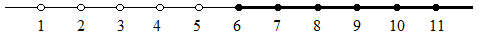
\includegraphics[width=4.46in,height=0.43in]{capitulos/conjuntos_numericos/media/image11.png}
	\end{Center}
\end{figure}
~~
b) 
\begin{figure}[H]
	\begin{Center}
		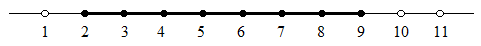
\includegraphics[width=4.4in,height=0.48in]{capitulos/conjuntos_numericos/media/image12.png}
	\end{Center}
\end{figure}
~~
c)
\begin{figure}[H]
	\begin{Center}
		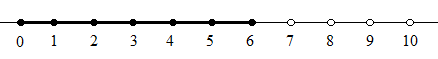
\includegraphics[width=4.56in,height=0.61in]{capitulos/conjuntos_numericos/media/image13.png}
	\end{Center}
\end{figure}
~~
d)
\begin{figure}[H]
	\begin{Center}
		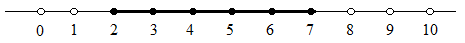
\includegraphics[width=4.84in,height=0.45in]{capitulos/conjuntos_numericos/media/image14.png}
	\end{Center}
\end{figure}
~~
e)
\begin{figure}[H]
	\begin{Center}
		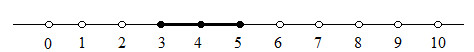
\includegraphics[width=4.94in,height=0.54in]{capitulos/conjuntos_numericos/media/image15.png}
	\end{Center}
\end{figure}
~~
f)
\begin{figure}[H]
	\begin{Center}
		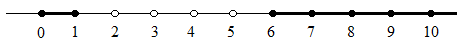
\includegraphics[width=4.83in,height=0.5in]{capitulos/conjuntos_numericos/media/image16.png}
	\end{Center}
\end{figure}
~~
	\ansitem{} a) Sim, b) Sim, c) Sim, mas em geral, é um número fracionário d) Sim e) Sim, mas em geral, é um número fracionário.

    \ansitem{} Não.

	\ansitem{} Não existe.

	\ansitem{} a)Sim, b) Não, c) Sim, e d) Não.

\end{respostas}

\begin{respostas}{3}
	\ansitem{} a) 3.~~~~ b) -25.~~ ~ c) -9.~~~~ d) -1.~~~~~ e) -2.~~~~ f) 35.~~~~~ g) 0.~~ ~ h) -22.~ ~  i) -8. ~~~~ j) 10.

	\ansitem{} R$\$$  -850,00.

	\ansitem{} a) 50 – 30 = 20.\quad b) 100 – 40 = 60.  \quad c) -100 + 50 = -50.\quad d) -200 – 70 = -270.

	\ansitem{} + 21ºC.

	\ansitem{} – 10ºC.

	\ansitem{} 220m.

	\ansitem{} Sim, (–2).

	\ansitem{} \( 6/2=~3   \in \mathbb{Z};6/4 \notin  \mathbb{Z} \).  

\ansitem{} a)~16.~~~~~b)~-64.~~~ c)0.     d)~1.~~  ~~ e)~+25.~~~~f)~+16.~~~~g)-16.     h)-32.

\ansitem{}a) $ \pm $ ~3.~~~~b)~3.~~~~~~~c)~-3.~~~~d)~$ \pm $ ~2.~~~~e)~$ \pm $ ~2.~~~~ f)+2.      g)-2.       h)-4.
\end{respostas}

\begin{respostas}{4}
	\ansitem{} a) -1.\quad b) -11/10.~~~ \quad c) $\frac{1}{2}$.\quad  d)1. ~~~~~~ e)1/24.\quad f)1.

	\ansitem{} a)-1/2.\quad b)4/9.~~~~~~~ c)-13/2.\quad d)-1/5.~~~~~~~ e)30.\quad f)3/2.
\end{respostas}

\begin{respostas}{5}
	\ansitem{} a)3.\quad b)2/3.\quad \quad c)4.\quad d)2.\quad e)4.\quad f)5/3.

	\ansitem{}  Racionais.

	\ansitem{} a)  \( 2\sqrt[]{2} \) \quad b)  \( 2\sqrt[]{3} \) ~~~ \quad c)  \( 2\sqrt[3]{3} \) \quad \quad d)  \( 2\sqrt[4]{2} \) ~~~~~~~~~ e)  \( \frac{2\sqrt[]{3}}{3\sqrt[]{5}} \) \quad \quad f)  \( \frac{2\sqrt[3]{2}}{5} \) 

	\ansitem{}  Irracionais. 

	\ansitem{}  a)  \( \sqrt[]{12} \) \quad b)  \( \sqrt[3]{54} \) \quad \quad c)  \( \sqrt[]{98} \) \quad \quad d) \( ~\sqrt[3]{\frac{1}{2}} \) ~~~~~~~~~~ e)  \( \sqrt[]{\frac{9}{2}} \) ~~~~~~~~ f)  \( \sqrt[]{\frac{75}{4}} \) 

	\ansitem{} a)  \( 7\sqrt[]{3} \) \quad b)  \( -2\sqrt[]{\frac{1}{2}} \)  ~ ~~ c)  \( \sqrt[6]{500} \) \quad ~~~ d)  \( \sqrt[]{\frac{15}{2}} \) ~~~~ e)  \( 3\sqrt[3]{\frac{3}{8}} \) \quad f)  \( 21\sqrt[]{10} \) ~~~ g)  \( \sqrt[]{5} \) \quad h)  \( \sqrt[]{20} \) 

	\ansitem{}  a)  \( 8\sqrt[]{5} \) \quad b)  \( \sqrt[]{6}+\sqrt[]{10} \) ~~~  c)  \( 8\sqrt[]{3}-3\sqrt[]{2} \) \quad d)  \( 2 \) ~~~ \quad  e)  \( 14-6\sqrt[]{5} \) \quad ~~~~~ f)  \( -5 \) 

	\ansitem{} ~ a)  \( \frac{\sqrt[]{3}}{3} \) \quad b)  \( \frac{3\sqrt[]{2}}{2} \) ~~ ~ c)  \( \frac{7\sqrt[]{5}}{5} \) ~~~~~ d)  \( 6-3\sqrt[]{3} \) ~~~~ e)  \( -\sqrt[]{2}-\sqrt[]{3} \) \quad f)  \( \frac{-175-35\sqrt[]{3}}{22} \) 

	\ansitem{}São iguais.

	\ansitem{} Respectivamente:$\mathbb{N}, \mathbb{Z}, \mathbb{Z}, \mathbb{I}, \mathbb{Q}, \mathbb{N}, \mathbb{Z}, \mathbb{I}, \mathbb{Q}, \mathbb{Q}, \mathbb{Q}$.

	\ansitem{} Porque o conjunto dos números Inteiros ($\mathbb{Z}$) está contido no conjunto dos números Racionais ($\mathbb{Q}$).

	\ansitem{}  -15~é um número inteiro, mas também é racional, porque podemos escrevê-lo  na forma de fração: -30/2, por exemplo.

	\ansitem{} ~ a)  \( \frac{3}{10} \) \quad  b)  \( \frac{5}{9} \) ~~~~~~  c)  \( \frac{132}{100} \) \quad d)  \( \frac{7}{33} \) ~~~~~ ~ e)  \( \frac{4}{3} \) \quad \quad f)  \( \frac{340}{99} \) ~~ 

	\ansitem{}Porque é um número decimal periódico infinito.

	\ansitem{}Porque é um número decimal não periódico.

	\ansitem{} Devido~à equivalência de frações, pois   \( \frac{2}{3} \cdot \frac{2}{2}=\frac{4}{6} \).
	
	\ansitem{}
\begin{multicols}{10}
	
	a) \( \mathbb{Q} \)
	
	b) \( \mathbb{Q} \)
	
	c) \( \mathbb{N} \)
	
	d) \( \mathbb{Q} \)
	
	e) \( \mathbb{Q} \)
	
	f) \( \mathbb{Q} \)

	g) \( \mathbb{Q} \)
	
	h) \( \mathbb{Q} \)
	
	i) \( \mathbb{N} \)
	
	j) $\mathbb{R}$
\end{multicols}
	\ansitem{}
	a) \( A =  \{ x \in \mathbb{N}/ x < 6 \}  \) 

	b)  \( B =  \{ x \in \mathbb{Z}/ -4 < x < 3 \}  \) 

	c)  \( C =  \{ x \in \mathbb{R}\frac{}{}x \geq -3 \}  \) 

	d)  \( D =  \{ x \in \mathbb{R} / -3 < x < 5 \}  \) 

	e)  \( E =  \{ x \in \mathbb{R} / 3 > x> 5 \}  \) 

	\ansitem{}
a)

\begin{figure}[H]
	\begin{Center}
		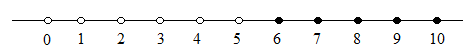
\includegraphics[width=3.92in,height=0.58in]{capitulos/conjuntos_numericos/media/image17.png}
	\end{Center}
\end{figure}

~~
 b)

\begin{figure}[H]
	\begin{Center}
		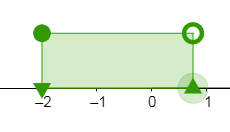
\includegraphics[width=3.83in,height=0.53in]{capitulos/conjuntos_numericos/media/image18.png}
	\end{Center}
\end{figure}

~~

 c)

\begin{figure}[H]
	\begin{Center}
		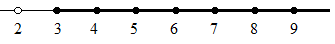
\includegraphics[width=3.49in,height=0.46in]{capitulos/conjuntos_numericos/media/image19.png}
	\end{Center}
\end{figure}

~~

d)

\begin{figure}[H]
	\begin{Center}
		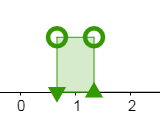
\includegraphics[width=4.17in,height=0.56in]{capitulos/conjuntos_numericos/media/image20.png}
	\end{Center}
\end{figure}

~~

 e)

\begin{figure}[H]
	\begin{Center}
		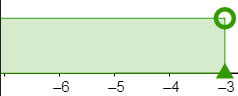
\includegraphics[width=4.38in,height=0.45in]{capitulos/conjuntos_numericos/media/image21.png}
	\end{Center}
\end{figure}

~~

 f)

\begin{figure}[H]
	\begin{Center}
		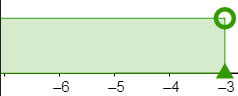
\includegraphics[width=4.38in,height=0.45in]{capitulos/conjuntos_numericos/media/image21.png}
	\end{Center}
\end{figure}

~~

 g)

\begin{figure}[H]
	\begin{Center}
		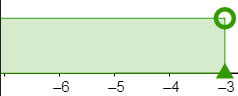
\includegraphics[width=4.38in,height=0.45in]{capitulos/conjuntos_numericos/media/image21.png}
	\end{Center}
\end{figure}

~~

 h)

\begin{figure}[H]
	\begin{Center}
		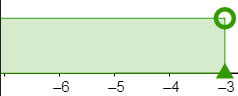
\includegraphics[width=4.38in,height=0.45in]{capitulos/conjuntos_numericos/media/image21.png}
	\end{Center}
\end{figure}

~~

\ansitem{} O número representado por este produto notável é racional (16).

\end{respostas}
